\chapter{Buscas em espaços de estados}
\label{cap:buscas}

\framebox[\textwidth]{
	\hspace{1em}
	\vbox{
		\textbf{Leitura obrigatória:}
		\begin{itemize}
			\item \cite{RusselAndNorvig2010} -- Cap. 3 (Resolução de problemas por meio de busca).
		\end{itemize}
		
		\textbf{Leitura complementar:}
		\begin{itemize}
			\item \cite{PooleAndMacworth2010} -- Cap. 3 (Searching for solutions).
		\end{itemize}
	}
}

\section{Agentes de resolução de problemas}

No Capítulo~\ref{cap:agentes-inteligentes} foi apresentado o conceito de agentes para a construção de sistemas inteligentes. Foram discutidas diferentes propriedades de ambientes e diferentes estruturas de agentes para operar sobre estes ambientes. O restante deste material apresenta conceitos, técnicas e abordagens de inteligência artificial que podem ser incorporadas nos agentes para obter um bom desempenho na execução de suas tarefas.

Em alguns casos, os agentes não possuem um mapeamento direto entre o estado observado e uma ação que satisfaça seu objetivo. O exemplo típico é um veículo autônomo que deve optar entre dois caminhos possíveis. Neste caso, se o agente conhece apenas o próximo ponto de cada caminho (e nenhum dos pontos é o destino da viagem), ele não terá escolha senão escolher aleatoriamente entre as opções. Em contrapartida, se o agente possui uma visão maior do seu ambiente, como um mapa da cidade, ele pode analisar qual caminho leva ao destino de sua viagem. Ou ainda, qual dos caminhos leva ao seu destino com o menor custo. Neste sentido, o agente está resolvendo o problema de chegar ao seu destino e, portanto, podemos classificá-lo como um agente que resolve problemas. Uma das formas de resolver problemas como a escolha de caminhos é através de algoritmos de \textbf{busca}, os quais são estudados neste capítulo.

\section{Formulação de problemas e soluções}

Um problema de busca pode ser definido por quatro componentes:
\begin{itemize}
	\item \textbf{Estado inicial}.
	\item \textbf{Função sucessor} ou \textbf{operador de estado}.
	\item \textbf{Teste de objetivo}.
	\item \textbf{Função de custo}.
\end{itemize}

O \textbf{estado inicial} define o estado em que a busca começa. A \textbf{função sucessor} retorna o conjunto de estados acessíveis a partir do estado atual. Em geral, costuma-se representar os sucessores como pares ordenados $\langle$\textit{ação}, \textit{sucessor}$\rangle$, ou seja, a ação que leva a determinado estado sucessor. Uma segunda abordagem consiste em utilizar \textbf{operadores de estado}, os quais operam sobre um estado, gerando o respectivo estado sucessor.

O \textbf{teste de objetivo} verifica se um determinado estado é aquele (ou um dos) que satisfaz o objetivo do agente. O \textbf{custo de caminho} atribui um custo numérico ao caminho que leva o estado inicial ao estado atual. Com isso, é possível determinar o custo de executar a sequência de ações para chegar no estado em questão.

\subsection{Exemplos de problemas}

Esta seção apresenta alguns exemplos de problemas típicos da área de inteligência artificial. Para a formalização dos problemas, é apresentada uma especificação dos estados possíveis, juntamente com a especificação dos componentes apresentados na seção anterior.

\subsubsection{Aspirador de pó}

Podemos modelar um problema de busca para o mundo do aspirador de pó apresentado no Capítulo~\ref{cap:agentes-inteligentes}.

\begin{itemize}
	\item \textbf{Estados:} cada estado é representado pela posição em que o robô se encontra e a situação (limpo ou sujo) dos dois quadrados. O robô tem $2$ possibilidades de posição, enquanto existem $2^2$ configurações possíveis de sujeira. Logo, existem $2 \times 2^2 = 8$ estados possíveis. O conjunto de estados possíveis é chamado de \textbf{espaço de estados}.
	
	\item \textbf{Estado inicial:} qualquer estado pode ser designado como estado inicial.
	
	\item \textbf{Função sucessor:} as ações possíveis do robô são: \textit{esquerda} (L), \textit{direita} (R) e \textit{aspirar} (S). Estas ações levam a novos estados ou permanecem no mesmo. O espaço de estados completo é apresentado na Figura~\ref{fig:espaco-estados-aspirador}.
	
	\item \textbf{Teste de objetivo:} verifica se todos os quadrados estão limpos.
	
	\item \textbf{Custo de caminho:} cada passo custa $1$, portanto, o custo do caminho é o número de passos realizados.
\end{itemize}

\begin{figure}[h]
	\centering
	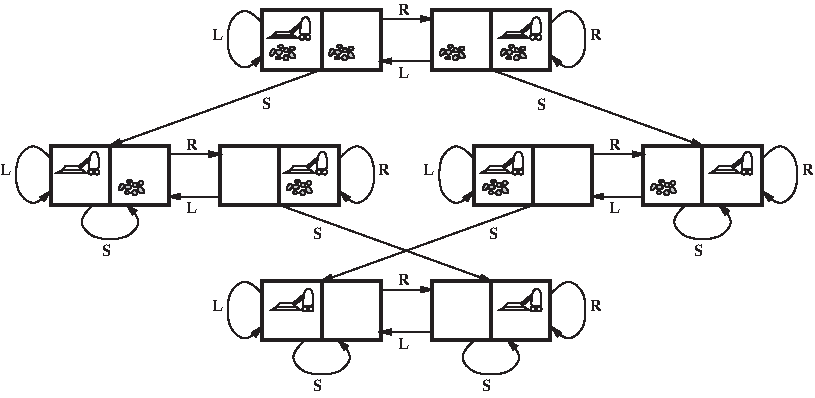
\includegraphics[width=\textwidth]{img/espaco-estados-aspirador}
	\caption{Espaço de estados para o mundo do aspirador de pó}
	\label{fig:espaco-estados-aspirador}
\end{figure}

\subsubsection{Quebra-cabeça de 8 peças}

O quebra-cabeça de 8 peças consiste em um tabuleiro de tamanho $3 \times 3$ com 8 peças numeradas e um espaço vazio. O objetivo é deslizar as peças pelo espaço vazio, de modo a ordená-las de forma crescente. A Figura~\ref{fig:quebra-cabeca-8-pecas} apresenta um exemplo do jogo com as peças embaralhadas e um exemplo com as mesmas ordenadas. É possível definir diferentes configurações de ordenação como estado objetivo.

\begin{itemize}
	\item \textbf{Estados:} cada estado especifica a posição de cada peça no tabuleiro e, consequentemente, o espaço vazio.
	
	\item \textbf{Estado inicial:} qualquer estado pode ser designado como estado inicial.
	
	\item \textbf{Função sucessor:} gera os estados válidos a partir das ações \textit{esquerda}, \textit{direita}, \textit{acima} e \textit{abaixo}, que podem er aplicadas à qualquer peça do jogo.
	
	\item \textbf{Teste de objetivo:} verifica se o estado corresponde à configuração desejada (conforme estado objetivo da Figura~\ref{fig:quebra-cabeca-8-pecas}).
	
	\item \textbf{Custo de caminho:} cada passo custa $1$, portanto, o custo do caminho é o número de passos realizados.
\end{itemize}

\begin{figure}[h]
	\centering
	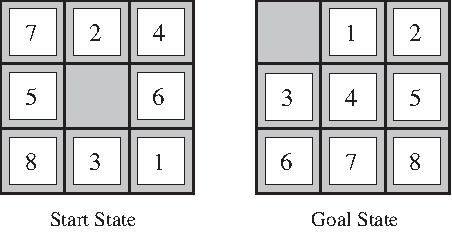
\includegraphics[width=0.5\textwidth]{img/quebra-cabeca-8-pecas}
	\caption{Exemplos de instâncias do quebra-cabeça de 8 peças}
	\label{fig:quebra-cabeca-8-pecas}
\end{figure}

\subsubsection{Problema das 8 rainhas}

O problema das 8 rainhas consiste em posicionar oito rainhas em um tabuleiro de xadrez\footnote{Existem variações com $n$ rainhas em tabuleiros $n \times n$.}, de tal forma que nenhuma rainha possa se atacar. Sabe-se que uma rainha pode atacar movimentando-se na linha, coluna ou na diagonal, um número qualquer de casas. A Figura~\ref{fig:exemplo-problema-8-rainhas} mostra um exemplo de posicionamento que não satisfaz o objetivo, pois as rainhas dos cantos superior esquerdo e inferior direito podem se atacar.

\begin{itemize}
	\item \textbf{Estados:} qualquer disposição de $0$ a $8$ rainhas no tabuleiro.
	
	\item \textbf{Estado inicial:} nenhuma rainha no tabuleiro.
	
	\item \textbf{Função sucessor:} colocar uma rainha em qualquer quadrado vazio.
	\begin{itemize}
		\item Uma abordagem que reduz o espaço de estados consiste em permitir a inserção de uma rainha apenas se o quadrado não estiver sob ataque.
	\end{itemize}
	
	\item \textbf{Teste de objetivo:} $8$ rainhas no tabuleiro sem que nenhuma possa se atacar.
	
	\item \textbf{Custo de caminho:} cada passo custa $1$, portanto, o custo do caminho é o número de passos realizados.
\end{itemize}

\begin{figure}[h]
	\centering
	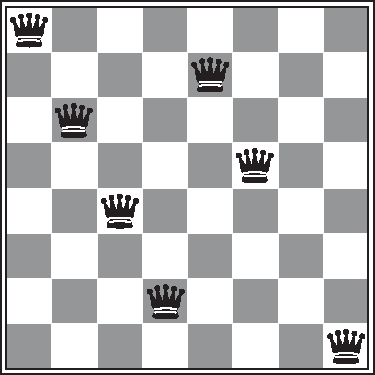
\includegraphics[width=0.5\textwidth]{img/exemplo-problema-8-rainhas}
	\caption{Exemplo de instância do problema das 8 rainhas}
	\label{fig:exemplo-problema-8-rainhas}
\end{figure}

\subsubsection{Roteamento}

Um dos problemas mais comuns é a definição de rotas, seja para veículos, pacotes em redes, aviões, etc. Consideremos o roteamento de veículos, tarefa similar à realizada por dispositivos GPS. A rede viária (mapa) é representada por um grafo, onde os vértices representam os pontos (cidades, por exemplo), enquanto os arcos representam caminhos de um ponto a outro (vias, por exemplo). A Figura~\ref{fig:grafo-cidades-roteamento} apresenta um grafo que representa o mapa de cidades da Romênia. O problema do roteamento consiste em encontrar o caminho de menor custo (também chamado de menor caminho ou caminho mínimo) entre uma origem e um destino. Por exemplo: qual o melhor caminho de \textit{Arad} até \textit{Bucharest}. Perceba que os arcos possuem valores associados, os quais representam o custo de viajar de um ponto a outro. Este grafo pode ser populado com diferentes custos, como distância, tempo de viagem, consumo de combustível, custo monetário, etc.

\begin{itemize}
	\item \textbf{Estados:} um estado é representado por um vértice (ou seja, uma cidade) acessível a partir do vértice de origem.
	
	\item \textbf{Estado inicial:} vértice de origem.
	
	\item \textbf{Função sucessor:} retorna o conjunto de vértices adjacentes do vértice atual. Ou seja, os vértices que possuam arcos com o vértice atual (comumente chamados de vizinhos).
	
	\item \textbf{Teste de objetivo:} verifica se o vértice atual é o vértice de destino.
	
	\item \textbf{Custo de caminho:} consiste no somatório dos custos dos arcos utilizados na rota.
\end{itemize}

\begin{figure}[h]
	\centering
	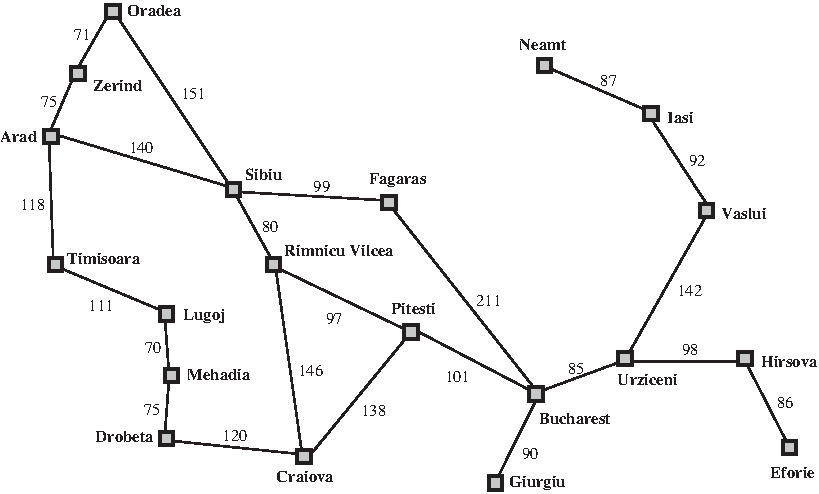
\includegraphics[width=\textwidth]{img/grafo-cidades-roteamento}
	\caption{Grafo das cidades da Romênia para o roteamento de veículos}
	\label{fig:grafo-cidades-roteamento}
\end{figure}

\subsection{Estratégia básica de busca}

A estratégia para solução destes problemas consiste em buscar no espaço de estados, algum estado que satisfaça o objetivo desejado (definido pelo teste de objetivo). Alguns problemas possuem uma única solução, isto é, um único estado que satisfaz o objetivo. Outros problemas, no entanto, possuem diferentes soluções, cada uma com seu respectivo custo. Finalmente, existem problemas para os quais qualquer estado é uma solução. Nos dois últimos casos, a estratégia de busca consiste em encontrar a melhor solução, ou seja, aquela que apresenta o menor custo. Esta solução é chamada de \textbf{solução ótima}.

Para realizar esta busca, deve-se partir do estado inicial e, através das ações disponíveis, caminhar para novos estados até encontrar um estado que satisfaça o objetivo. Para isso, criaremos uma \textbf{árvore de busca}, cujo nó raiz é o estado inicial, enquanto os nós filhos são os estados acessíveis mediante a realização das ações disponíveis. A Figura~\ref{fig:arvore-busca-roteamento} apresenta a árvore que busca uma rota entre as cidades de \textit{Arad} e \textit{Bucharest}, conforme o mapa apresentado na Figura~\ref{fig:grafo-cidades-roteamento}.

\begin{figure}[h]
	\centering
	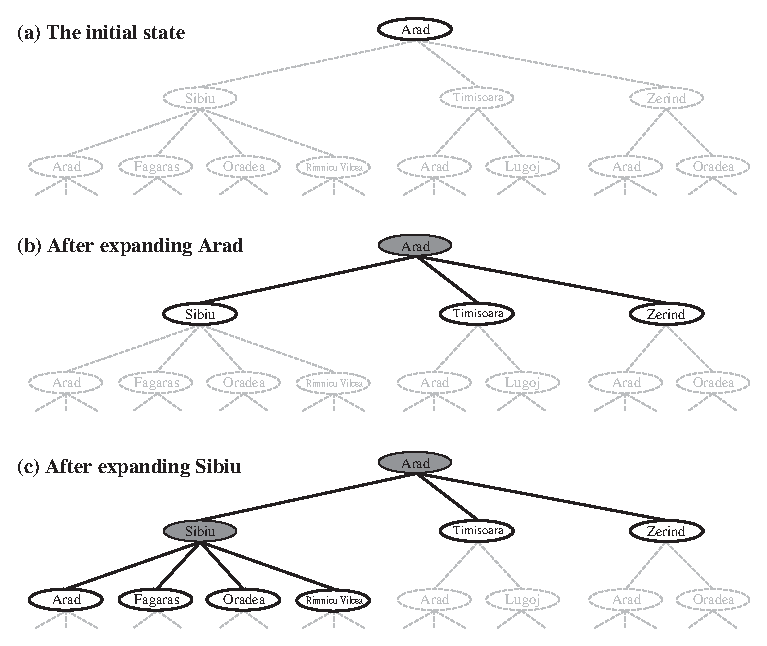
\includegraphics[width=\textwidth]{img/arvore-busca-roteamento}
	\caption{Árvore de busca para o problema de roteamento entre cidades da Romênia}
	\label{fig:arvore-busca-roteamento}
\end{figure}

A cada iteração, o algoritmo de busca deve verificar se o estado atual satisfaz o objetivo. No passo \texttt{(a)} da Figura~\ref{fig:arvore-busca-roteamento}, o estado atual consiste na cidade de origem, que é o estado inicial. Este nó é então expandido e os estados vizinhos são obtidos (através da função sucessor), o que é apresentado no momento \texttt{(b)}. O próximo estado é selecionado (\textit{Sibiu}). Como não satisfaz o objetivo, o nó é expandido \texttt{(c)}. A busca é executada até que o estado desejado (\textit{Bucharest}) é encontrado, ou quando se esgotam os vértices e a solução não é encontrada, caso em que o algoritmo deve retornar \texttt{falha}. O Algoritmo~\ref{alg:estrategia-basica-busca} apresenta um pseudocódigo para esta estratégia básica de busca.

\begin{algorithm}[h]
	\DontPrintSemicolon
	\Entrada{\textit{problema}, \textit{estratégia de seleção}}
	\Saida{\textit{solução}}
	
	\Inicio{
		\Repita{não haverem mais nós para expandir}{
			Seleciona um nó para expansão de acordo com \textit{\underline{estratégia de seleção}}\;
			\Se{nó contém um estado objetivo}{
				\Retorna{\textit{Solução correspondente}}
			}
			\Senao{
				Expandir o nó e adicionar os sucessores à árvore de busca\;
			}
		}
		\Retorna{\texttt{falha}}
	}
	
	\caption{Pseudocódigo para a estratégia básica de busca}
	\label{alg:estrategia-basica-busca}
\end{algorithm}

O que difere diferentes abordagens de busca é a estratégia de seleção de nós. Na Figura~\ref{fig:arvore-busca-roteamento}, o nó \textit{Arad} foi expandido para três filhos: \textit{Sibiu}, \textit{Timisoara} e \textit{Zerind}. No passo seguinte, o nó \textit{Sibiu} foi expandido para quatro novas cidades. Logo, o próximo passo poderia selecionar nós ainda não visitados do nível 2 ou do nível 3 da árvore. A estratégia de seleção de nós pode fazer com que o algoritmo tenha um desempenho melhor ou pior, de acordo com o problema tratado.

\textbf{Observação:} é importante diferenciar o \textit{espaço de estados} da \textit{árvore de busca}. No exemplo do roteamento, existem apenas 20 cidades no mapa e, portanto, 20 estados diferentes. Por outro lado, a árvore de busca é muito maior, pois consiste nos diferentes caminhos possíveis que podem ser feitos nesta rede. A árvore pode ser inclusive infinita, que é o caso deste problema de roteamento, uma vez que permite caminhos cíclicos\footnote{É claro que um bom algoritmo de busca deve evitar ciclos e, dessa forma, podar a árvore de busca.}. A árvore de busca é também chamada de \textbf{espaço de busca}.

\insertspace

Cada nó da árvore de busca é representado por uma estrutura de dados contendo:
\begin{itemize}
	\item \textbf{Estado:} o estado a que o nó corresponde.
	\item \textbf{Nó pai:} o nó da árvore que gerou esse nó.
	\item \textbf{Ação:} a ação que foi aplicada ao pai para gerar esse nó.
	\item \textbf{Custo:} o custo $g(n)$ do caminho desde o estado inicial até o nó.
	\item \textbf{Profundidade:} o número de passos ao longo do caminho, desde o estado inicial.
\end{itemize}

\insertspace

Finalmente, os diferentes algoritmos de busca são avaliados em função de quatro critérios:
\begin{itemize}
	\item \textbf{Completude:} o algoritmo oferece a garantia de encontrar uma solução, caso ela exista?
	
	\item \textbf{Otimalidade:} o algoritmo oferece a garantia de encontrar a solução ótima?
	
	\item \textbf{Complexidade de tempo:} quanto tempo ele leva para encontrar uma solução?
	
	\item \textbf{Complexidade de espaço:} quanta memória é necessária para executar a busca?
\end{itemize}

\insertspace

A complexidade em tempo e espaço é medida em função de alguns parâmetros do problema:
\begin{itemize}
	\item \textbf{Fator de ramificação $b$:} quantidade máxima de sucessores que qualquer nó pode gerar.
	
	\item \textbf{Profundidade $d$:} profundidade (nível) do nó meta mais próximo do inicial.
	
	\item \textbf{Comprimento máximo $m$:} comprimento máximo de qualquer caminho no espaço de estados.
\end{itemize}

\section{Algoritmos de busca cega}
\label{sec:busca-cega}

Os algoritmos de busca em árvore se dividem em duas categorias: busca cega e busca informada. A busca cega não possui qualquer informação sobre o problema, exceto sua definição. Com isso, ela tem que percorrer a árvore, verificando se o estado satisfaz o objetivo. Por outro lado, a busca informada consegue determinar o quanto um estado se aproxima do estado objetivo e, com isso, guiar a busca por ramos mais promissores da árvore, bem como descartar ramos ruins. Esta seção apresenta alguns algoritmos de busca cega que podem ser aplicados a qualquer problema\footnote{Ser aplicável a qualquer problema não significa que sua performance seja suficiente para resolver o problema.}.

\subsection{Busca em largura}

A busca em largura aplica uma estratégia onde o nó raiz é expandido, então todos os sucessores são expandidos, depois os sucessores dos sucessores, e assim por diante. Em outras palavras, todos os nós de uma dada profundidade na árvore de busca são expandidos, antes que todos os nós do nível seguinte sejam expandidos. A Figura~\ref{fig:busca-largura} mostra esta estratégia na exploração de uma árvore binária simples. Perceba que os nós \texttt{B} e \texttt{C} são expandidos antes dos nós \texttt{D}, \texttt{E}, \texttt{F} e \texttt{G}.

\begin{figure}[h]
	\centering
	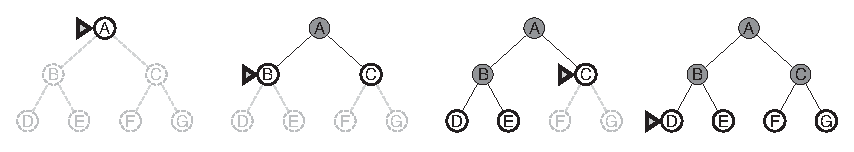
\includegraphics[width=\textwidth]{img/busca-largura}
	\caption{Busca em largura em uma árvore binária simples}
	\label{fig:busca-largura}
\end{figure}

A estratégia de busca em largura pode ser implementada utilizando uma estrutura de dados do tipo fila (FIFO -- \textit{first-in-first-out}) para armazenar os nós que ainda não foram expandidos. Em cada expansão, os filhos do nó expandido são inseridos na fila e, portanto, serão expandidos antes que seus filhos. O Algoritmo~\ref{alg:busca-largura} apresenta o pseudocódigo para uma busca em largura.

\begin{algorithm}[h]
	\DontPrintSemicolon
	\Entrada{\textit{nó inicial}}
	\Saida{\textit{solução}}
	
	\Inicio{
		Fila abertos $\gets \emptyset$\;
		abertos.add(inicial)\;
		\Enqto{abertos $\neq \emptyset$}{
			Nó atual $\gets$ abertos.remove()\;
			\Se{testeObjetivo(atual.estado)}{
				\Retorna{solução(atual)}
			}
			abertos.add(sucessores(atual))\;
		}
		
		\Retorna{\texttt{falha}}
	}
	
	\caption{Pseudocódigo para uma busca em largura}
	\label{alg:busca-largura}
\end{algorithm}

A busca em largura é \textit{completa}, pois sempre encontra uma solução caso ela exista. No entanto, esta solução não é garantidamente a melhor, portanto a busca não é ótima. Caso os custos sejam não-decrescentes à profundidade da solução, como um custo fixo igual para todas as ações, então a busca em largura é ótima, pois a melhor solução é a que se encontra no menor nível possível.

O problema da busca em largura é a complexidade de tempo e espaço. Considerando um fator de ramificação $b$ e uma profundidade $d$, cada nível $i$ expande $b^{i+1}$ nós da árvore de busca. No pior caso, a solução estará no último nó do nível $d$, o qual não será expandido. Portanto, no último nível a busca expande $b^{d+1} - b$ nós. Com isso, temos a complexidade\footnote{Esta complexidade pode ser diminuída para $O(b^d)$ se a verificação do nó possuir o estado objetivo ou não for realizada na sua geração, em vez de realizar na sua expansão.}
$$
b + b^2 + b^3 + \ldots + b^d + (b^{d+1} - b) = O(b^{d+1}).
$$

Considerando um fator de ramificação $b = 10$, que $10.000$ nós podem ser gerados por segundo e que um nó ocupa $1.000$\,bytes de espaço de armazenamento, a Tabela~\ref{tab:complexidade-busca-largura} mostra a quantidade de nós, o tempo gasto e a memória utilizada para uma busca em largura com diferentes valores de profundidade $d$. Muitos problemas apresentam estas características, o que nos leva a concluir que o tempo e a memória são os problemas críticos da busca em largura. Não temos computadores com memória na ordem de terabytes, por exemplo.

\begin{table}[h]
	\centering
	\setlength{\tabcolsep}{20pt}
	\begin{tabular}{rrrr}
		\hline
		\textbf{Profundidade} & \textbf{Nós} & \textbf{Tempo} & \textbf{Memória} \\
		\hline
		$2$ & $1100$ & $0,11$ segundo & $1$ megabyte \\
		$4$ & $111.100$ & $11$ segundos & $106$ megabytes \\
		$6$ & $10^7$ & $19$ minutos & $10$ gigabytes \\
		$8$ & $10^9$ & $31$ horas & $1$ terabyte \\
		$10$ & $10^{11}$ & $129$ dias & $101$ terabytes \\
		$12$ & $10^{13}$ & $35$ anos & $10$ petabytes \\
		$14$ & $10^{15}$ & $3.523$ anos & $1$ exabyte \\
		\hline
	\end{tabular}
	
	\caption{Desempenho de uma busca em largura em número de nós, tempo e espaço}
	\label{tab:complexidade-busca-largura}
\end{table}

\subsection{Busca em profundidade}

Diferente da anterior, a busca em profundidade sempre expande o nó mais profundo no conjunto de nós a serem expandidos. Esta estratégia é ilustrada na Figura~\ref{fig:busca-profundidade}, onde observamos que a busca desce os níveis na árvore até que o nó não tenha sucessores (\texttt{A} -- \texttt{B} -- \texttt{D} -- \texttt{H} $\ldots$). Quando os nós expandidos não tiverem mais sucessores a serem expandidos, eles não serão mais utilizados e podem ser removidos da memória, o que garante um consumo muito menor de espaço.

\begin{figure}[h]
	\centering
	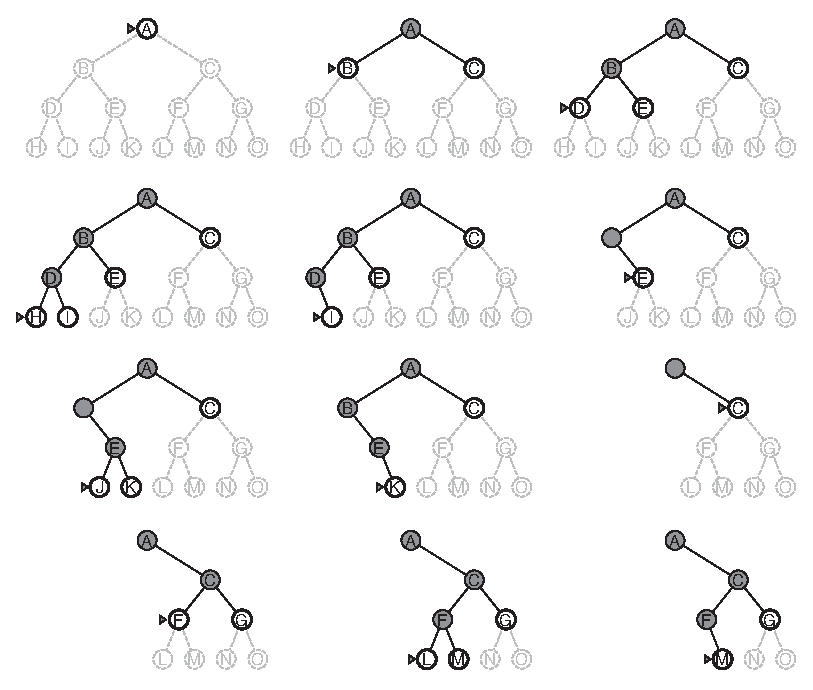
\includegraphics[width=\textwidth]{img/busca-profundidade}
	\caption{Busca em profundidade em uma árvore binária simples}
	\label{fig:busca-profundidade}
\end{figure}

Para implementar este comportamento, podemos utilizar uma estrutura de dados do tipo pilha (LIFO -- \textit{last-in-first-out}) para armazenar os nós que ainda não foram expandidos. Com isso, o último nó aberto é inserido na pilha e, portanto, será o primeiro a ser selecionado para expansão. O pseudocódigo para a busca em profundidade consiste em trocar a fila por uma pilha no Algoritmo~\ref{alg:busca-largura}. A busca em profundidade é completa somente se a árvore não é infinita, o que não é garantido em muitos problemas. Apesar de ser completa em árvores finitas, a busca não é ótima, pois uma solução sub-ótima pode ser encontrada em um primeiro ramo da árvore.

Como os ramos completamente explorados podem ser removidos da memória, a busca em profundidade só precisa armazenar um único caminho desde a raiz até um nó de folha, juntamente com os nós irmãos não expandidos restantes de cada nó no caminho. Considerando um fator de ramificação $b$ e uma profundidade máxima $m$, a busca em profundidade possui complexidade de espaço de $bm + 1 = O(bm)$. Considerando o mesmo cenário da Tabela~\ref{tab:complexidade-busca-largura} e supondo que nós da mesma profundidade do nó objetivo não têm sucessores, a busca em profundidade para $d = 12$ utilizaria $118$ kilobytes, ao invés de $10$ petabytes da busca em largura.

A complexidade de tempo de uma busca em profundidade depende da profundidade máxima $m$ da árvore de busca. Logo, podemos definir a complexidade de tempo como $O(b^m)$. Caso a árvore seja infinita (por conta de estados repetidos), a busca não terminaria sua execução e algum mecanismo de poda deve ser adotado.

\subsection{Busca em profundidade limitada}

Uma abordagem comum é limitar o nível de profundidade, gerando uma \textbf{busca em profundidade limitada}. Definindo um limite de profundidade $l$, nós no nível $l$ serão tratados como se não tivessem sucessores. A busca passa a ser incompleta se $l < d$, o que é um fator importante uma vez que na maioria dos problemas não se conhece $d$ \textit{a priori}. O Algoritmo~\ref{alg:busca-profundidade-limitada} apresenta um pseudocódigo para uma busca em profundidade limitada.

\begin{algorithm}[h]
	\DontPrintSemicolon
	\Entrada{\textit{nó inicial}, \textit{limite de profundidade} $l$}
	\Saida{\textit{solução}}
	
	\Inicio{
		Pilha abertos $\gets \emptyset$\;
		abertos.add(inicial)\;
		\Enqto{abertos $\neq \emptyset$}{
			Nó atual $\gets$ abertos.remove()\;
			\Se{testeObjetivo(atual.estado)}{
				\Retorna{solução(atual)}
			}
			
			\Se{atual.profundidade $< l$}{
				abertos.add(sucessores(atual))\;
			}
		}
		
		\Retorna{\texttt{falha}}
	}
	
	\caption{Pseudocódigo para uma busca em profundidade limitada}
	\label{alg:busca-profundidade-limitada}
\end{algorithm}

Mesmo com a seleção de um limite $l > d$, a busca em profundidade limitada não garante otimalidade. No entanto, suas complexidades de tempo e espaço são ainda menores, pois a exploração é feita em parte da árvore de busca. A busca em profundidade tradicional pode ser vista como uma busca em profundidade limitada com $l = \infty$.

A complexidade da busca é medida, obviamente, em função do limite $l$. A complexidade de tempo é é $O(b^l)$, enquanto a complexidade de espaço é $O(bl)$.

\subsection{Busca em profundidade iterativa}

Uma vez que não se conhece \textit{a priori} um valor adequado para o limite de profundidade $l$, a busca em profundidade iterativa tenta encontrar o melhor valor durante a sua execução. Para isso, o algoritmo aumenta gradativamente o valor de $l$, iniciando por 0 e incrementando em 1, até encontrar uma solução, que ocorre quando $l = d$. Em outras palavras, esta abordagem combina a busca em profundidade com a busca em largura. O Algoritmo~\ref{alg:busca-profundidade-iterativa} apresenta um pseudocódigo para a busca em profundidade iterativa.

\begin{algorithm}[h]
	\DontPrintSemicolon
	\Entrada{\textit{nó inicial}}
	\Saida{\textit{solução}}
	
	\Inicio{
		\Para{$l \gets 0$ \textbf{até} $\infty$}{
			solução $\gets$ BUSCA-PROFUNDIDADE-LIMITADA(\textit{inicial}, $l$)\;
			\Se{solução $\neq$ \texttt{falha}}{
				\Retorna{solução}
			}
		}
	}
	
	\caption{Pseudocódigo para uma busca em profundidade iterativa}
	\label{alg:busca-profundidade-iterativa}
\end{algorithm}

\begin{figure}[h]
	\centering
	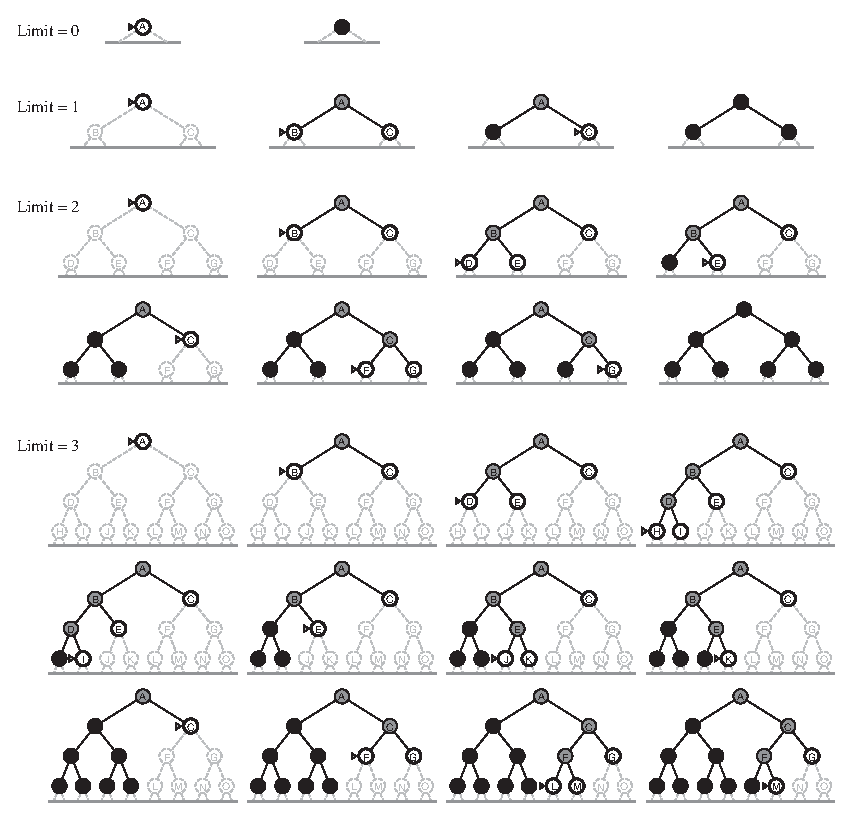
\includegraphics[width=0.995\textwidth]{img/busca-profundidade-iterativa}
	\caption{Busca em profundidade iterativa em uma árvore binária simples}
	\label{fig:busca-profundidade-iterativa}
\end{figure}

%\clearpage

A Figura~\ref{fig:busca-profundidade-iterativa} ilustra o funcionamento de uma busca em profundidade iterativa. No limite 0, apenas a raiz é analisada. No limite 1, a raiz é expandida e o primeiro nível é analisado. Quando os níveis aumentam, a estratégia de seleção de nós é idêntico ao de uma busca em profundidade, mas os nós mais rasos já foram explorados em iterações anteriores. Logo, este algoritmo faz uma busca em largura sem a necessidade de manter os nós em memória, isto é, utiliza os benefícios de ambas abordagens.

A busca em profundidade iterativa é completa, pois encontra uma solução, caso ela exista. Da mesma forma que ocorre na busca em largura, esta abordagem é ótima se o custo for não-decrescente (uniforme, por exemplo) ao nível de profundidade. Apesar de parecer desperdício gerar os mesmos estados repetidamente em diferentes iterações, o maior número de estados (em maiores níveis de profundidade) são gerados poucas vezes. De fato, o nível $d$ é gerado uma só vez, o nível $d+1$ é gerado duas vezes, e assim por diante. Logo, temos a seguinte complexidade de tempo:
$$
(d)b + (d - 1)b^2 + \ldots + (1)b^d = O(b^d).
$$

Comparando a complexidade da busca em profundidade iterativa ($O(b^d)$) com a busca em largura ($O(b^{d+1} - b)$), percebemos que a busca em largura é mais complexa, pois gera alguns nós de profundidade $d+1$. Como resultado, a busca em profundidade iterativa é mais rápida e, na maioria dos casos, é o algoritmo de busca preferido quando existe um espaço de busca grande e a profundidade da solução não é conhecida.

\subsection{Busca bidirecional}

A ideia da busca bidirecional é executar duas buscas em paralelo. A primeira busca é simples e explora os nós a partir do estado inicial, conforme visto até o momento. A segunda busca utiliza o estado objetivo como estado inicial, explorando a árvore de busca a partir dele. Quando as duas buscas encontrarem um nó em comum, o caminho desde o estado inicial até o estado objetivo é traçado. A ideia geral desta busca é expressa na Figura~\ref{fig:busca-bidirecional}. A motivação desta busca é que $b^{d/2} + b^{d/2} < b^d$. Isto é, a soma das áreas dos dois círculos é menor que a área de um grande círculo partindo do estado inicial até encontrar o estado objetivo. 

\begin{figure}[h]
	\centering
	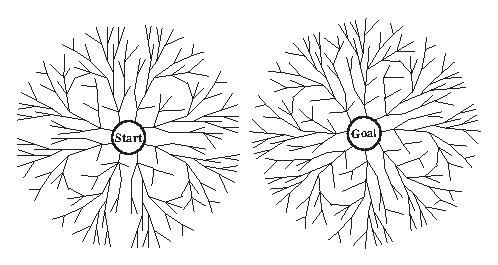
\includegraphics[width=0.8\textwidth]{img/busca-bidirecional}
	\caption{Ideia geral da busca bidirecional}
	\label{fig:busca-bidirecional}
\end{figure}

No momento da geração de nós, cada busca verifica se os nós não estão na lista de nós a serem explorados da outra busca. Em caso positivo, é encontrada uma solução. Se um problema possui solução na profundidade $d = 6$ e são executadas duas buscas em largura, então no pior caso cada busca expande todos os nós da profundidade 3, exceto um. Para $b = 10$, isso significa $22.200$ nós gerados, em comparação com $11.111.100$ nós gerados por uma busca em largura.

Como a busca de um nó na outra árvore pode ser feito em tempo constante, a complexidade de tempo de uma busca bidirecional é $O(b^{d/2})$. A complexidade de espaço é definida pelo armazenamento de pelo menos uma das árvores em memória, o que leva à mesma complexidade de $O(b^{d/2})$. Caso ambas as buscas forem em largura e os passos tiverem custo uniforme, então a busca é completa e ótima. Diferentes buscas podem sacrificar uma ou as duas características.

A dificuldade deste método está na exploração do espaço de estados a partir do estado objetivo. Nem sempre é possível determinar os predecessores de um estado, ou seja, os estados-pai possíveis. Isso faz com que a busca bidirecional não possa ser aplicada a qualquer problema.

\subsection{Comparação entre as abordagens}

A Tabela~\ref{tab:comparacao-busca-cega} resume a avaliação dos diferentes métodos de busca cega apresentados neste capítulo.

\begin{table}[h]
	\centering
	\small
	\begin{tabular}{l|L{2.5cm}L{2.5cm}L{2.5cm}L{2.5cm}}
		\hline
		\textbf{Busca} & \textbf{Completa} & \textbf{Ótima} & \textbf{Tempo} & \textbf{Espaço} \\
		\hline
		
		Largura & Sim & Sim\tablefootnote{Desde que o custo do passo seja não-decrescente ao nível de profundidade.} & $O(b^{d+1})$ & $O(b^{d+1})$ \\
		
		Profundidade & Não & Não & $O(b^m)$ & $O(bm)$ \\
		
		Profundidade limitada & Não & Não & $O(b^l)$ & $O(bl)$ \\
		
		Profundidade iterativa & Sim & Sim\tablefootnote{Desde que o custo do passo seja não-decrescente ao nível de profundidade.} & $O(b^d)$ & $O(bd)$ \\
		
		Bidirecional & Sim\tablefootnote{Desde que ambas as buscas sejam em largura.} & Sim\tablefootnote{Se ambas as buscas sejam em largura e os custos dos passos sejam todos idênticos.} & $O(b^{d/2})$ & $O(b^{d/2})$ \\
		\hline
		
	\end{tabular}
	\caption{Comparação de diferentes estratégias de busca cega}
	\label{tab:comparacao-busca-cega}
\end{table}

\section{Algoritmos de busca informada}

A Seção~\ref{sec:busca-cega} apresentou alguns algoritmos de busca que não possuem nenhuma informação do problema, exceto sua definição. Com isso, estes métodos exploram a árvore de busca, verificando cada estado gerado seguindo alguma estratégia genérica. Estes algoritmos não são aplicáveis a problemas reais, pois eles comumente são muito grandes e complexos. Com isso, a busca cega não consegue encontrar a solução em tempo razoável com os recursos de memória existentes. Para resolver este problema, podemos utilizar informações do problema para guiar a busca, explorando regiões promissoras da árvore de busca. Estes algoritmos são classificados como busca informada.

Para isso, utilizaremos uma \textbf{função de avaliação} $f(n)$ que determina o custo de um nó da árvore de busca. Dessa forma, a busca pode selecionar os nós de menor custo para exploração. Esta função é definida como:
$$
f(n) = g(n) + h(n),
$$
em que $n$ é um nó da árvore de busca, $g(n)$ é o \textbf{custo do caminho} desde o nó inicial até $n$ e $h(n)$ é chamada \textbf{função heurística}.

O custo do caminho é armazenado em cada nó da árvore e é proveniente do custo da execução das ações que levam até um determinado estado, conforme apresentado nas seções anteriores. A função heurística deve ser determinada pelo projetista e mede (ou estima) a distância do nó atual ($n$) até o nó objetivo.

\subsection{Busca uniforme}

Uma primeira abordagem consiste em selecionar o nó cujo caminho até ele seja o menor possível. Em outras palavras, consideramos $f(n) = g(n)$. Esta abordagem é chamada de busca uniforme e garante a otimalidade, desde que os custos sejam positivos. O Algoritmo~\ref{alg:busca-informada} mostra o pseudocódigo para uma busca informada, onde a lista de nós abertos é ordenada em função de $f(n)$ (linha 2), isto é, selecionando sempre o menor valor (linha 5).

\begin{algorithm}[h]
	\DontPrintSemicolon
	\Entrada{\textit{nó inicial}}
	\Saida{\textit{solução}}
	
	\Inicio{
		ListaOrdenada abertos $\gets \emptyset$\;
		abertos.add(inicial)\;
		\Enqto{abertos $\neq \emptyset$}{
			Nó atual $\gets$ abertos.removeFirst()\;
			\Se{testeObjetivo(atual.estado)}{
				\Retorna{solução(atual)}
			}
			abertos.add(sucessores(atual))\;
		}
		
		\Retorna{\texttt{falha}}
	}
	
	\caption{Pseudocódigo para uma busca informada}
	\label{alg:busca-informada}
\end{algorithm}

A busca uniforme garante que, quando um nó é selecionado para expansão, foi encontrado o menor caminho até ele. Ao retomar o problema do roteamento entre as cidades da Romênia (Figura~\ref{fig:grafo-cidades-roteamento-2}), consideremos a tarefa de ir de \textit{Sibiu} para \textit{Bucharest}. Ao expandir o nó \textit{Sibiu}, são abertos os nós \textit{Fagaras}, com custo de 99 e \textit{Rimnicu Vilcea}, com custo de 80. O nó \textit{Rimnicu Vilcea} é selecionado para expansão, adicionando as cidades de \textit{Pitesti} (custo de $80 + 97 = 177$) e \textit{Craiova} (custo de $80 + 146 = 226$). Com isso, o menor custo passa a ser \textit{Fagaras}, que é selecionado, abrindo o nó de \textit{Bucharest}, com custo de $99 + 211 = 310$. Apesar de este ser o nó destino, existem caminhos em aberto que possuem custo menor que 310. Ou seja, pode ser que encontremos um caminho com custo menor que o encontrado até o momento. Por isso, a busca uniforme só termina quando garantidamente não existe um caminho de menor custo.

Seguindo a busca, o nó de menor custo é \textit{Pitesti} (custo de $80 + 97 = 177$), que é selecionado, abrindo o nó \textit{Bucharest} com custo de $177 + 101 = 278$. Perceba que encontramos um caminho com menor custo que o anterior. Além disso, os caminhos em aberto possuem todos um custo maior que 278. Logo, o próximo nó selecionado é \textit{Bucharest} e garantimos que o caminho de menor custo foi encontrado.

\begin{figure}[h]
	\centering
	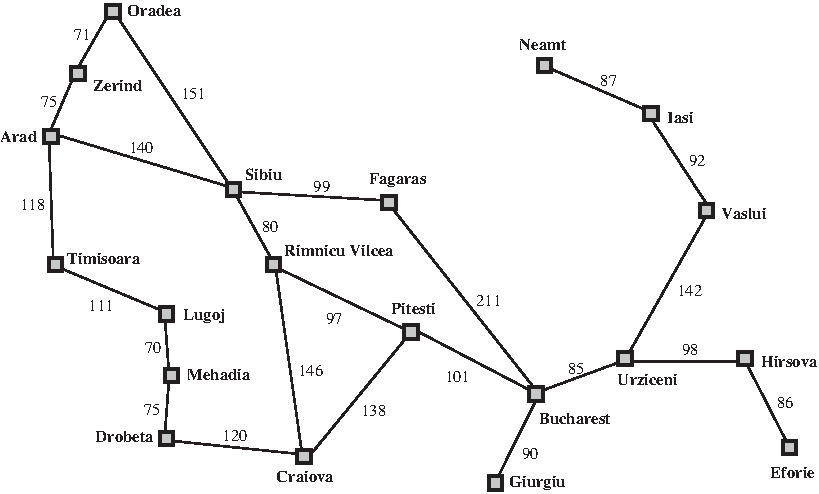
\includegraphics[width=\textwidth]{img/grafo-cidades-roteamento}
	\caption{Grafo das cidades da Romênia para o roteamento de veículos}
	\label{fig:grafo-cidades-roteamento-2}
\end{figure}

Apesar de ser um algoritmo ótimo quando os custos são positivos, esta estratégia demora para convergir, pois não descarta nenhum caminho (ramo da árvore) até ter a certeza de que não pode produzir um caminho melhor. Por exemplo, uma grande sequência de passos pequenos sempre será explorada até descobrir que adiante existe um passo gigante que elimina este caminho da solução. Além disso, se tivermos algum arco com custo igual a zero, a busca pode ficar presa em um laço infinito ao selecionar sempre o mesmo nó para expansão.

\subsection{Busca gulosa}

A busca gulosa (\textit{greedy search}) é também conhecida por busca gulosa de melhor escolha e utiliza a função heurística como guia para uma busca mais rápida. Ou seja, a busca gulosa define $f(n) = h(n)$ e expande o nó que apresenta o menor $f(n)$, até encontrar a solução. Seu funcionamento é o mesmo apresentado no Algoritmo~\ref{alg:busca-informada}, considerando a nova função $f(n)$. Em resumo, é a estratégia contrária à busca uniforme, pois ao invés de usar o custo do caminho do início até o nó $n$, utiliza o custo estimado do nó $n$ até o objetivo. 

Consideremos o problema de roteamento entre as cidades da Romênia (Figura~\ref{fig:grafo-cidades-roteamento-2}), partindo de \textit{Arad} com destino em \textit{Bucharest}. Como a busca não conhece o grafo completo, não é possível utilizar a distância real de cada cidade até o destino \textit{Bucharest}. Portanto, consideremos como função heurística $h(n)$ a distância em linha reta de cada cidade até \textit{Bucharest}. Estes valores são apresentados na Tabela~\ref{tab:distancias-cidades-bucareste}. Exemplo: $h($\textit{Arad}$) = 366$.

\begin{table}[b!]
	\centering
	\begin{tabular}{lr|lr}
		\hline
		\textbf{Cidade} & \textbf{Distância} & \textbf{Cidade} & \textbf{Distância}\\
		\hline
		Arad & 366 & Mehadia & 241 \\
		Bucharest & 0 & Neamt & 234 \\
		Craiova & 160 & Oradea & 380 \\
		Drobeta & 242 & Pitesti & 100 \\
		Eforie & 161 & Rimnicu Vilcea & 193 \\
		Fagaras & 176 & Sibiu & 253 \\
		Giurgiu & 77 & Timisoara & 329 \\
		Hirsova & 151 & Urzineci & 80 \\
		Iasi & 226 & Vaslui & 199 \\
		Lugoj & 244 & Zerind & 374 \\
		\hline
	\end{tabular}
	
	\caption{Distância de cada cidade até Bucharest -- para função heurística}
	\label{tab:distancias-cidades-bucareste}
\end{table}

O funcionamento da busca gulosa para o problema de roteamento na Romênia é ilustrado na Figura~\ref{fig:execucao-busca-gulosa}. O nó inicial é \textit{Arad}, que possui $f(n) = h(n) = 366$. A expansão desse nó gera os nós \textit{Sibiu}, \textit{Timisoara} e \textit{Zerind}. A busca seleciona o nó \textit{Sibiu}, pois apresenta menor $f(n)$. Sua expansão gera mais quatro nós, dos quais \textit{Fagaras} é selecionado, pois apresenta o menor $f(n)$. Finalmente, a expansão de \textit{Fagaras} gera \textit{Bucharest}, que é o nó objetivo. A busca encontra, portanto, a solução para o problema.

\insertspace

\begin{figure}[h]
	\centering
	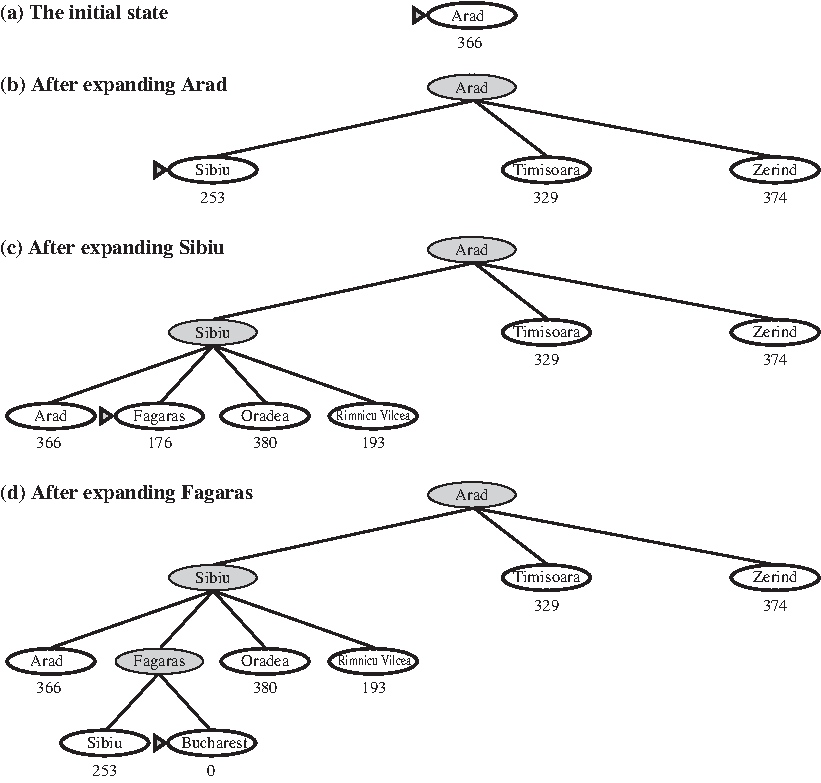
\includegraphics[width=\textwidth]{img/execucao-busca-gulosa}
	\caption{Execução de uma busca gulosa para roteamento entre cidades da Romênia}
	\label{fig:execucao-busca-gulosa}
\end{figure}

A busca gulosa não é ótima. Perceba que existe um caminho de menor custo (\textit{Arad} -- \textit{Sibiu} -- \textit{Rimnicu Vilcea} -- \textit{Pitesti}). Por conta da gulosidade (ambição) da busca, ela ignora regiões da árvore de busca que parecem ser mais custosas mas levam a uma solução melhor. Além disso, a busca não é completa caso nenhuma estratégia de poda seja utilizada, pois mesmo em espaços de estados finitos a árvore de busca pode ser infinita (ciclos) e a busca nunca encontra uma solução\footnote{Mesma situação da busca em profundidade.}.

\subsection{Busca A*}

A busca A* (A estrela) utiliza simultaneamente as estratégias adotadas nas buscas uniforme e gulosa. Isto é, considera o custo do caminho e o custo futuro estimado. Com isso, a busca A* considera caminhos com menor expectativa de custo, mas evita caminhos que já estejam muito caros. A função $f(n) = g(n) + h(n)$ pode ser vista como o custo estimado da solução que passa pelo nó $n$. Com isso, se garante a otimalidade da busca uniforme, mas a árvore não precisa ser explorada exaustivamente. O funcionamento da busca A* é idêntico ao Algoritmo~\ref{alg:busca-informada} com a lista de nós ordenada pela nova função $f(n)$.

A execução do algoritmo de busca A* para o roteamento entre cidades da Romênia é apresentada na Figura~\ref{fig:execucao-busca-a-estrela}. Observe que a busca considera $f(n) = g(n) + h(n)$ para a seleção de vértices. A cidade de \textit{Bucharest} aparece como candidata à seleção da etapa \texttt{(e)}. No entanto, o caminho passando por \textit{Rimnicu Vilcea} -- \textit{Pitesti} parece mais promissor, pois possui menor $f(n)$. Logo, a busca A* seleciona o nó \textit{Pitesti}, encontrando um caminho mais curto.

\begin{figure}[h]
	\centering
	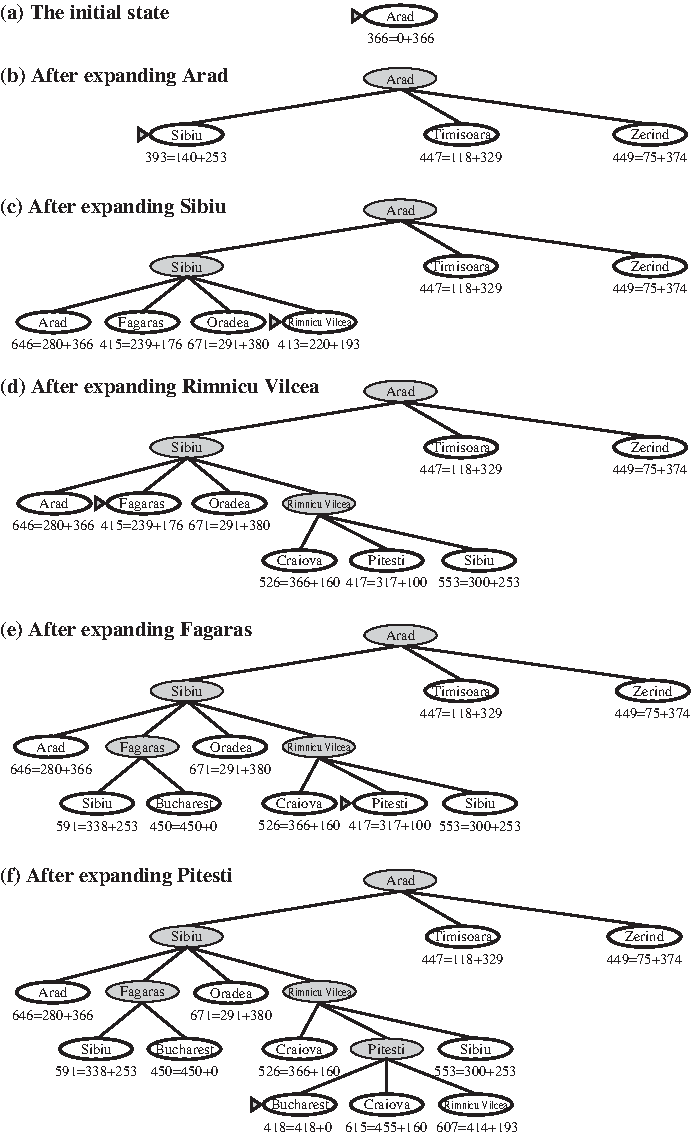
\includegraphics[width=0.9\textwidth]{img/execucao-busca-a-estrela}
	\caption{Execução de uma busca A* para roteamento entre cidades da Romênia}
	\label{fig:execucao-busca-a-estrela}
\end{figure}

A busca A* é completa, pois evita ciclos, uma vez que considera o custo passado. Obviamente, esta condição é verdadeira somente se os custos nas arestas forem maiores que zero. A busca A* é também ótima, desde que a função heursítica $h(n)$ seja \textbf{admissível}. A função é admissível caso ela \textbf{nunca superestime} o custo para alcançar o objetivo (dizemos que a função deve ser otimista). Em outras palavras, o custo estimado pela função heurística deve ser menor ou igual ao custo real. Caso a busca superestime o custo, ela pode descartar a solução ótima por calcular um custo superior ao real.

No caso do roteamento entre cidades da Romênia, a função heurística é admissível, pois a distância entre duas cidades não pode ser menor que a distância de uma linha reta entre elas. Logo, $h(n)$ não pode ser uma superestimativa e a busca é ótima para este problema.

\section{Recursos disponíveis}

Existem vários sites e aplicações com o objetivo de ensinar e esclarecer os algoritmos de busca em árvores, como o Visualgo~\footnote{\url{https://visualgo.net/en}} e as ferramentas disponibilizadas pelo professor David Galles~\footnote{\url{https://www.cs.usfca.edu/~galles/visualization/Algorithms.html}}. Além disso, a ferramenta Web de \textit{Graph Searching}~\footnote{\url{http://aispace.org/search}} da plataforma AIspace~\footnote{\url{http://www.aispace.org}}. Finalmente, existem bibliotecas que implementam os algoritmos de busca em árvore, como a disponibilizada pelo professor Jomi Hübner~\footnote{\url{http://jomi.das.ufsc.br/ia/busca/buscaJava/index.html}}.

\clearpage

\section{Exercícios}

\resetexercisenumbering

\begin{exercise}
Defina com suas próprias palavras os seguintes termos: estado, espaço de estados, árvore de busca, nó de busca, objetivo, ação, modelo de transição e fator de ramificação.
\end{exercise}

\begin{exercise}
Qual é a diferença entre um estado do mundo, uma descrição do estado e um nó de busca? Por que é útil essa distinção?
\end{exercise}

\begin{exercise}
Suponha que dois amigos vivam em cidades de locais diferentes no mapa da Romênia. Podemos mover cada amigo de cada vez simultaneamente para uma cidade vizinha no mapa. A quantidade de tempo necessário para se deslocar da cidade $i$ à vizinha $j$ é igual à distância $d(i,j)$ entre as cidades, mas a cada vez que o amigo chega primeiro deve
esperar até o outro chegar (e telefonar para o primeiro do celular) antes que comece a próxima vez de se movimentarem. Queremos que os dois amigos se encontrem o mais rápido possível.

\begin{enumerate}[a.]
	\item Escreva uma formulação detalhada para esse problema de busca (será útil definir alguma notação formal).
	
	\item Seja $D(i,j)$ a distância em linha reta entre as cidades $i$ e $j$. Qual das seguintes funções heurísticas é admissível? (i) $D(i,j)$, (ii) $2 \cdot D(i,j)$ e (iii) $D(i,j) / 2$.
	
	\item Há mapas completamente conectados para os quais não existe solução?
	
	\item Há mapas em que todas as soluções requerem que um amigo visite a mesma cidade duas vezes?
\end{enumerate}
\end{exercise}

\begin{exercise}
Forneça uma formulação completa do problema para cada um dos seguintes itens. Escolha a formulação suficientemente precisa para ser implementada.

\begin{enumerate}[a.]
	\item Usando apenas 4 cores, colorir um mapa plano de tal forma que duas regiões adjacentes não tenham a mesma cor.
	
	\item Um macaco com 30 cm está em uma sala onde tem algumas bananas suspensas em um teto de 80\,cm. Ele gostaria de pegar as bananas. A sala contém dois engradados móveis e escaláveis com 30\,cm de altura que podem ser empilhados.
	
	\item Existem três jarras que medem 12, 8 e 3 galões e uma torneira de água. As jarras podem ser enchidas ou esvaziadas uma da outra ou para o chão. Medir exatamente um galão, somente com essas operações.
\end{enumerate}
\end{exercise}

\begin{exercise}
Este exercício explora a aplicação dos algoritmos de busca quando existem custos negativos nos caminhos.

\begin{enumerate}[a.]
	\item Suponha que as ações possam ter custos negativos arbitrariamente grandes; explique por que essa possibilidade forçaria qualquer algoritmo ótimo a explorar todo o espaço de estados.
	
	\item Ajudaria se insistíssemos no fato de que os custos dos passos devem ser maiores ou iguais a alguma constante negativa $c$?
	
	\item Suponha que um conjunto de ações forme um laço no espaço de estados de modo que a cada execução dessas ações em alguma ordem não resulte em mudança no estado. Se todas essas ações tiverem custo negativo, qual será a implicação desse fato sobre o comportamento ótimo de um agente em tal ambiente?
	
	\item É possível imaginar facilmente ações com custo negativo alto, até mesmo em domínios como o de roteamento. Por exemplo, alguns trechos da estrada poderiam ter belas paisagens que superem de longe os custos normais em termos de tempo e combustível. Explique, em termos precisos, dentro do contexto de busca em espaços de estados, por que os seres humanos não dirigem indefinidamente em ciclos por belos cenários e explique como definir o espaço de estados e ações para roteamento, de forma que agentes artificiais também possam evitar ciclos repetitivos.
\end{enumerate}
\end{exercise}

\begin{exercise}
O problema de missionários e canibais é normalmente enunciado como a seguir. Três missionários e três canibais estão em um lado de um rio, juntamente com um barco que pode levar uma ou duas pessoas. Descubra um meio de fazer todos atravessarem o rio sem deixar que um grupo de missionários de um lado fique em número menor que o número de canibais nesse mesmo lado do rio.

\begin{enumerate}[a.]
	\item Formule o problema precisamente, fazendo apenas as especificações necessárias para assegurar uma solução válida. Faça um diagrama do espaço de estados completo.
	
	\item Implemente e resolva o problema de forma ótima, utilizando um algoritmo de busca apropriado. É uma boa ideia verificar a existência de estados repetidos?
	
	\item Por que você imagina que as pessoas têm dificuldades para resolver esse quebra-cabeça, considerando que o espaço de estados é tão simples?
\end{enumerate}
\end{exercise}

\begin{exercise}
Uma ação tal como \textit{Ir para Sibiu} consiste realmente em uma longa sequência de ações mais refinadas: ligar o carro, soltar o freio, acelerar para a frente, etc. Ter ações compostas desse tipo reduz o número de passos em uma sequência de soluções, reduzindo assim o tempo de busca. Suponha que tomemos essa lógica ao extremo, construindo ações supercompostas de todas as sequências possíveis de ações \textit{Ir}. Assim, cada instância do problema é resolvida por uma única ação supercomposta, como \textit{Ir para Sibiu -- Ir para Rimnicu Vilcea -- Ir para Pitesti -- Ir para Bucareste} . Explique como a busca trabalharia nessa formulação. Essa é uma abordagem prática para acelerar a resolução do problemas?
\end{exercise}

\begin{exercise}
Quais das seguintes alternativas são falsas e quais são verdadeiras? Explique suas respostas.

\begin{enumerate}[a.]
	\item A busca em profundidade sempre expande pelo menos tantos nós quanto a busca A* com uma heurística admissível.
	
	\item $h(n) = 0$ é uma heurística admissível para o quebra cabeças de 8 peças.
	
	\item Em robótica, A* não é útil porque as percepções, estados e ações são contínuas.
	
	\item A busca em largura é completa mesmo se os custos de passos iguais a zero forem permitidos.
	
	\item Assuma que a torre pode se mover em um tabuleiro de xadrez qualquer quantidade de quadrados em linha reta, verticalmente ou horizontalmente, mas não pode pular sobre as peças. A distância de Manhattan é uma heurística admissível para o problema de movimentar a torre do quadrado \texttt{A} para o \texttt{B} no menor número de movimentos.
\end{enumerate}
\end{exercise}

\begin{exercise}
Considere um espaço de estados onde o estado inicial é o número $1$ e cada estado $k$ tem dois sucessores: números $2k$ e $2k + 1$.

\begin{enumerate}[a.]
	\item Represente a porção do espaço de estados para os estados de 1 a 15.
	
	\item Suponha que o estado objetivo seja 11. Liste a ordem em que os nós serão visitados pela busca em largura, busca em profundidade limitada com o limite 3 e busca de aprofundamento iterativo.
	
	\item Como a busca bidirecional funcionaria nesse problema? Qual é o fator de ramificação em cada direção?
	
	\item A resposta ao item \texttt{(c)} sugere uma reformulação do problema que permitiria resolver o problema de ir do estado 1 para um determinado estado objetivo com quase nenhuma busca?
	
	\item Chame a ação que vai de $k$ para $2k$ de Esquerda e a ação de $k$ que vai para $2k + 1$ de Direita. É possível encontrar um algoritmo que devolva a solução desse problema absolutamente sem nenhuma busca?
\end{enumerate}
\end{exercise}

\begin{exercise}
Faça passo a passo a execução de uma busca A* aplicada para o problema de chegar a \textit{Bucharest} a partir de \textit{Lugoj} utilizando a distância heurística em linha reta. Isto é, mostre a sequência de nós que o algoritmo vai considerar e a pontuação $f$, $g$ e $h$ para cada nó.
\end{exercise}

\begin{exercise}
Considere o problema do quebra cabeça de 8 peças, formalizado neste capítulo. Implemente os seguintes algoritmos de busca:

\begin{itemize}
	\item Busca em largura
	\item Busca em profundidade
	\item Busca A*
\end{itemize}

Faça um relatório mostrando o desempenho de cada algoritmo: custo do caminho encontrado até a solução, quantidade de vértices visitados, quantidade de vértices armazenados na memória a cada iteração e tempo de execução.
\end{exercise}

\begin{exercise}
Utilize a biblioteca de algoritmos de busca disponibilizada em \url{http://jomi.das.ufsc.br/ia/busca/buscaJava/index.html}. Esta biblioteca implementa os principais algoritmos discutidos neste material e apresenta a documentação de uso desses algoritmos. Aplique os algoritmos abaixo para o problema das $N$-Rainhas (com diferentes valores de $N$) e analise o seu desempenho.

\begin{itemize}
	\item Busca em largura
	\item Busca em profundidade
	\item Busca A*
	\item Busca subida da montanha
\end{itemize}
\end{exercise}

\begin{exercise}
Utilize a biblioteca de algoritmos de busca disponibilizada em \url{http://jomi.das.ufsc.br/ia/busca/buscaJava/index.html} para o problema das Torres de Hanoi. Uma descrição do problema pode ser consultada em \url{https://goo.gl/X4fVMM}. Um jogo matemático do problema pode ser consultado em \url{http://www.somatematica.com.br/jogos/hanoi/}. Implemente variantes com diferentes números de discos. Compare o desempenho dos algoritmos neste problema.
\end{exercise}